\section{Baseline}

We did a svd directly to the full version
(\ie, none sparse algorithms used) of the matrix,
which took
\begin{equation}
    t_0=21403
\end{equation}
 seconds, about $6$ hours.
The eigenvalues was shown in Figure~\ref{fig:eig}.
We can see that the dominating values only take a small proportion.
For example,
known that the largest eigenvalue is 7383.58,
there are only 81 eigenvalues that are larger than 500,
and when we set the threshold to be 1000,
merely 15 of them survive.
% > 500: 81
% > 600: 48
% > 700: 33
% > 800: 24
% > 900: 19
% > 1000: 15
So it is reasonable to use a low-rank matrix to approximate the data.
We also show the distribution of eigenvalues that are larger than 500
in Figure~\ref{fig:eig}.

\begin{figure}[!ht]
	\centering
	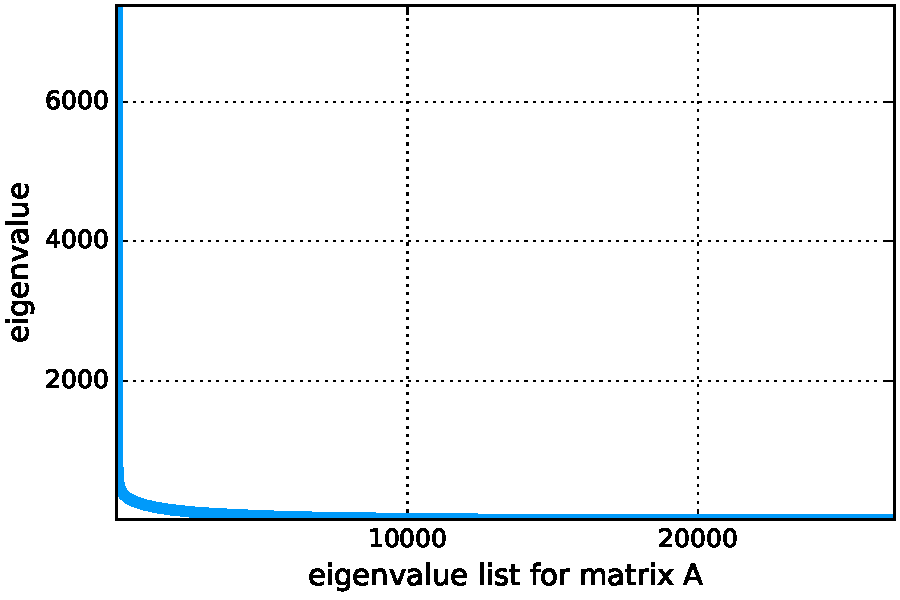
\includegraphics[width=0.48\textwidth]{fig/eigs.pdf}
    \hskip 0.2cm
	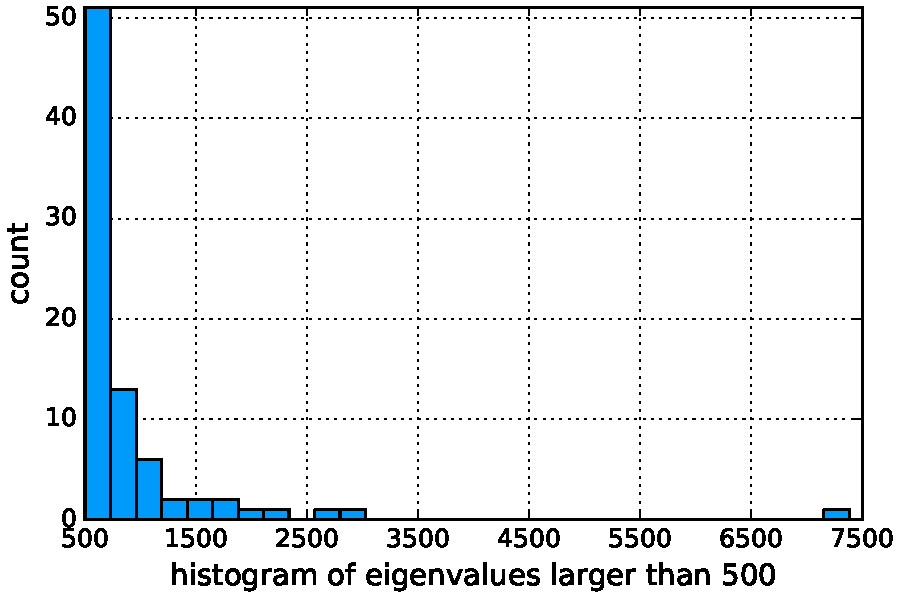
\includegraphics[width=0.48\textwidth]{fig/eig_large.pdf}
	\caption{\small
  		\textbf{Left}: Eigenvalues of matrix $A$.
          They are sorted for visualization.
          We can see a small portion of very large values.
        \textbf{Right}: Detailed distribution for large eigenvalues.}
	\label{fig:eig}
\end{figure}

To find a gook rank $k$,
we plot the curve of error energy (squared Frobenius norm) v.s. rank $k$
in Figure~\ref{fig:rank}.
Since there are quick methods (like sparse svd function \textit{svds()} in Julia)
computing part of the svd given rank $k$,
The running time of svds() is shown in Figure~\ref{fig:rank}.
We can see that when $k=128$,
the relative error energy is around 50\% and
the running time for svds in this setting is
\begin{equation}
    t_1=111.4
\end{equation}
seconds.
We will set
\begin{equation}
    k=128
\end{equation}
in the following experiments since it captures half of the energy
as well as keeps a relative small rank at the same time.
The Frobenius norm
\begin{equation}
	\| A - A_128 \| = 11622.2.
\end{equation}

\begin{figure}[!ht]
	\centering
	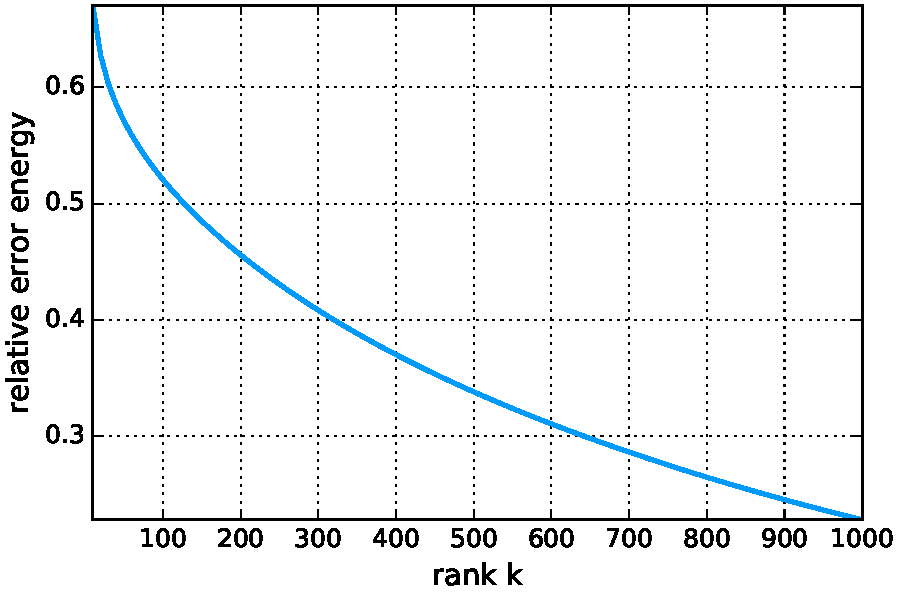
\includegraphics[width=0.48\textwidth]{fig/ranks.pdf}
    \hskip 0.2cm
	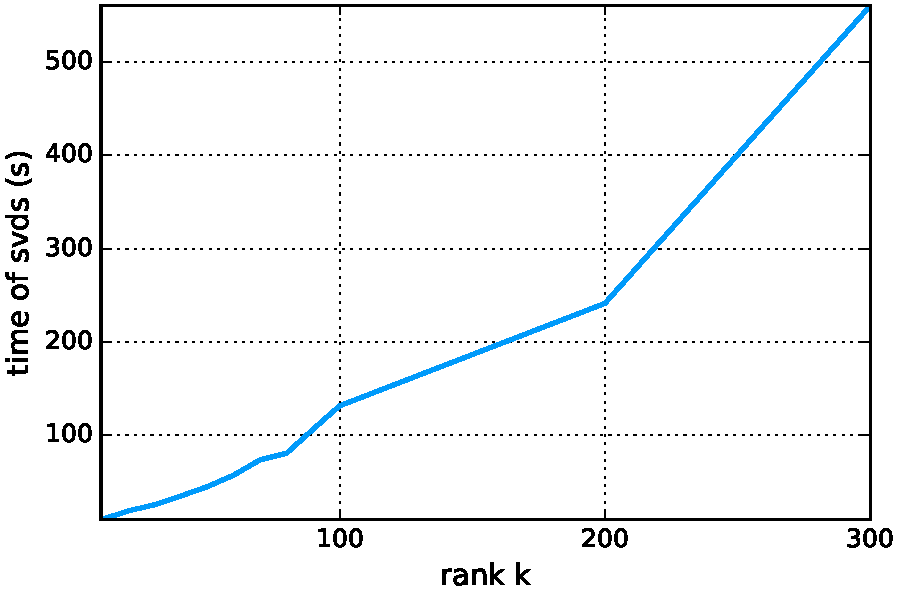
\includegraphics[width=0.48\textwidth]{fig/ranks_time.pdf}
	\caption{\small
  		\textbf{Left}: Relative errors of the best rank $k$ approximation to $A$
          which are measured in the Frobenius norm squared.
        \textbf{Right}: The running time of sparse svd, svds(), in different $k$.}
	\label{fig:rank}
\end{figure}
